\documentclass{article}
\usepackage{ctex}
\usepackage{amsmath}
\usepackage{amssymb}
\usepackage{amsfonts}
\usepackage{pstricks,pst-eps}
\usepackage{tikz}
\usepackage{multirow}
\usepackage{longtable}
\usepackage{graphicx}
\usepackage{subfigure}
\usepackage{listings}

%opening
\title{基于C语言的样条曲线拟合及Yin集布尔代数实现}
\author{徐圣泽}
\usepackage[a4paper,left=25mm,right=25mm,top=25mm,bottom=25mm]{geometry}  
\newcommand{\enabstractname}{Abstract}
\newcommand{\cnabstractname}{摘要}
\newenvironment{enabstract}{%
	\par\small
	\noindent\mbox{}\hfill{\bfseries \enabstractname}\hfill\mbox{}\par
	\vskip 2.5ex}{\par\vskip 2.5ex}
\newenvironment{cnabstract}{%
	\par\small
	\noindent\mbox{}\hfill{\bfseries \cnabstractname}\hfill\mbox{}\par
	\vskip 2.5ex}{\par\vskip 2.5ex}

\begin{document}
	
	\maketitle

	\section{前言}
	本篇文章基于样条曲线和Yin集的理论,通过编写软件包实现了曲线的样条拟合、Yin集及其布尔代数的有效表示。我认为此次大作业的重点在于将两部分的理论联系在一起写出有实际数学和物理意义的程序,事实证明每个部分的程序都是彼此关联着的,且都具有一定的实际价值。
	
	我在题中要求的三个编程部分给出了相应的算法,并且在本文展现了算法的思路、测试过程以及最终结果,最终利用算法写出程序,实现结果的呈现。
	
	第一部分样条曲线拟合的部分,我基于《计算方法引论》一书中的数学理论编写程序,并且实现了偏序关系的判断。对于第二部分布尔代数的实现,我采用了一种比较朴素的呈现方法,但严格来讲并未实现对Yin集合这一类的封闭运算,详细的实现过程会在后文进行阐述。
	\section{卡通图案的表示}
	\subsection{选定黑白卡通图}
	根据题目要求,选取了一个至少包含五个层次的黑白卡通图案。
	\begin{figure}[h]
		\centering
		\includegraphics[width=0.5\textwidth]{panda.jpeg}
		\caption{黑白卡通图案}
	\end{figure}
	\subsection{选取特征点}
	选取的黑白卡通图案共有13条边界曲线,利用MATLAB中\verb|grabit|功能,逐条选取特征点,存入文本文件中。
	\subsection{拟合样条曲线}
	\subsubsection{数学理论}
	设在区间$[a,b]$上取$n+1$个节点,给定节点上的函数值$f(x_i)=y_i$,现在构造三次样条插值函数$s(x)$满足下列条件:
	(1)$s(x_i)=y_i.$
	(2)在每个小区间$[x_i,x_{i+1}]$上是一个不高于三次的多项式.
	(3)$s(x)∈C_{[a,b]}^2$.
	假设在区间$[a,b]$上三次样条插值函数$s(x)$存在,并用$m_i$来表示$s(x)$在点$x_i$处的微商值,由于曲线通过点$(x_i,y_i)$,并且在每一个小区间$[x_i,x_{i+1}]$上满足条件:
	$$
	\begin{aligned}
		&s(x_i)=y_i,s(x_{i+1})=y_{i+1}\\
		&s'(x_i)=m_i,s'(x_{i+1})=m_{i+1}
	\end{aligned}
	$$
	
	故根据$Hermite$插值公式写出小区间$[x_i,x_i+1]$上的三次样条插值函数$s(x)$的计算公式:
	$$
	\begin{aligned}
		s(x)=&(1+2\frac{x-x_i}{x_{i+1}-x_i})(\frac{x-x_{i+1}}{x_i-x_{i+1}})^2y_i+(1+2\frac{x-x_{i+1}}{x_i-x_{i+1}})(\frac{x-x_i}{x_{i+1}-x_i})^2y_{i+1}
		\\&+(x-x_i)(\frac{x-x_{i+1}}{x_i-x_{i+1}})^2m_i+(x-x_{i+1})(\frac{x-x_i}{x_{i+1}-x_i})^2m_{i+1}
	\end{aligned}
	$$
	
	需要设法求出节点$x_i$处的微商值$m_i$,利用函数$s(x)$在节点$x_i$上二阶微商连续的性质,对$x$求微商并令$h_i=x_{i+1}-x_i$,不难得到:
	$$
	\begin{aligned}
	s''(x)=&(\frac{6}{h_i^2}-\frac{12}{h_i^3}(x_{i+1}-x))y_i+(\frac{6}{h_i^2}-\frac{12}{h_i^3}(x-x_i))y_{i+1}+
	\\
	&(\frac{2}{h_i}-\frac{6}{h_i^2}(x_{i+1}-x))m_i-(\frac{2}{h_i}-\frac{6}{h_i^2}(x-x_i))m_{i+1}
	\end{aligned}
	$$
	
	因此可以得到区间$[x_i,x_i+1]$上点$x_i$的右微商和左微商:
	$$
	\begin{aligned}
		&s''(x_i^+)=-\frac{6}{h_i^2}y_i+\frac{6}{h_i^2}y_{i+1}-\frac{4}{h_i}m_i-\frac{2}{h_i}m_{i+1}\\
		&s''(x_i^-)=\frac{6}{h_{i-1}^2}y_{i-1}-\frac{6}{h{i-1}^2}y_i+\frac{2}{h_{i-1}}m_{i-1}+\frac{4}{h_{i-1}}m_i
	\end{aligned}
	$$
	
	利用左微商等于右微商,可整理得到:
	$$
	\left\{
	\begin{aligned}
		&\alpha_i=\frac{h_{i-1}}{h_{i-1}+h_i}\\
		&\beta_i=3(\frac{1-\alpha_i}{h_{i-1}}(y_i-y_{i-1})+\frac{\alpha_i}{h_{i}}(y_{i+1}-y_i))
	\end{aligned}
	\right.
	$$
	
	同时得到方程组:
	$$
	(1-\alpha_i)m_{i-1}+2m_i+\alpha_im_{i+1}=\beta_i
	$$
	
	这是关于$n+1$个未知量的$n-1$个线性方程组,因此为了得到特定的一个解,还需要边界条件。下面每个算法都提供了一种边界条件的情形,补充了两个附加条件。
	
	\newpage
	\subsubsection{程序及结果}
	本程序定义了两个函数,分别用于处理边界条件为端点处一阶导已知和二阶导已知的情形,读取存放于文本文件的特征点坐标后,分别计算得到每条边界曲线每一小段样条曲线的参数,此处的参数即上面提到的未知数微商$m[i]$。
	
	\begin{figure}[!h]
		\centering
		\subfigure[1]{\includegraphics[width=0.45\textwidth]{c1.png}}
		\subfigure[2]{\includegraphics[width=0.45\textwidth]{c2.png}}
		\caption{程序运行结果}
	\end{figure}
	
	需要说明的是,上述结果采取的是自然边界条件,且首尾点坐标一致(即开始点也作为结束点,以此实现闭曲线)。利用MATLAB绘制相应曲线,并利用自带$spline$和$csape$函数检验程序输出参数的正确性(通过检验一些坐标根据程序输出表达式对应的函数值是否符合MATLAB的计算结果,事实证明程序是正确的)。
	\begin{figure}[h]
		\centering
		\includegraphics[width=0.8\textwidth]{plotcubic.png}
		\caption{样条拟合后的曲线}
	\end{figure}
	
	\newpage
	\subsection{判断偏序关系}
	\subsubsection{模型简化}
	在本部分我们需要判断几乎不相交的闭样条的偏序关系。根据相关理论,我们可以将问题化归为判断各闭合曲线之间的包含关系。
	
	首先,由题意知任意两条闭曲线是不相交的,因此只有包含、被包含、非包含三种关系。为判断两条曲线是否具有包含关系,只要判断一条曲线上的某点是否落在另一条曲线上或曲线包围成的区域内。
	
	在本题的求解过程中,我们可以简化问题模型,将所有闭曲线包围成的区域视作由特征点连线成的线性多边形。我们有两个原因足够说明此操作的合理性:1、在第二步我们为足够接近原图的样条曲线取了足够多的特征点;2、即使不视作线性多边形,我们也需要设置步长(后文会详细解释算法),很难做到逐点遍历。
	
	\subsubsection{射线法}
	假设此时已经有$\gamma_1$和$\gamma_2$两条边界。我们只需要检验两条曲线上的所有特征点是否同时满足上述条件。
	
	首先设计了第一种算法,分别遍历得到两条曲线横纵坐标的最大值和最小值,如果一条曲线的横、纵坐标的最大值比另一条曲线的横、纵坐标的最大值大,而最小值小,同时满足这四个条件,则此曲线必然包含于另一条曲线。
	
	此种算法已经能检验大多数情况,如下图左侧情形,但仍有少数情况无法被此算法正确判断,如右侧情形。
	\begin{figure}[h]
		\centering
		\subfigure[1]{\includegraphics[width=0.35\textwidth]{inside1.jpg}}
		\subfigure[2]{\includegraphics[width=0.35\textwidth]{inside2.jpg}}
		\caption{两种相似情形}
	\end{figure}
	
	为此我们必须设计出一种更合理的算法,能够适用于任何情况,下面我们采用射线法。考虑以下情形,已给定一闭合曲线,此时取定任意一个点,向任意方向作一射线,若此射线与曲线交点数为奇,则该点在区域内部,若交点数为偶,在该点在区域外部。下图中$O$和$J$对应上述两种情形。
	\begin{figure}[h]
		\centering
		\includegraphics[width=0.4\textwidth]{raymethod.png}
		\caption{射线法的两种情形}
	\end{figure}
	
	\newpage
	\subsubsection{程序及结果}
	原卡通图案的边界若尔当曲线标注如下。
	\begin{figure}[h]
		\centering
		\includegraphics[width=0.6\textwidth]{pandanote.jpg}
		\caption{卡通图案的若尔当曲线}
	\end{figure}

	我们的程序输出的是一个矩阵,矩阵第$i$行第$j$列($i\neq j$)的元素代表第$i$条曲线和第$j$条曲线的包含关系,$1$代表前者包含后者($\succeq$),$-1$代表被包含($\preceq$),$0$代表无包含关系。程序的运行结果如下:
	$$
	\left[
	\begin{array}{ccccccccccccc}
		0  & 1 & 1  & 1  & 1  & 1  & 1 & 1  & 1  & 1  & 1 & 1 & 1 \\
		-1 & 0 & 0  & 0  & 0  & 0  & 0 & 0  & 0  & 0  & 0 & 0 & 0 \\
		-1 & 0 & 0  & 1  & 1  & 1  & 1 & 1  & 1  & 1  & 1 & 1 & 1 \\
		-1 & 0 & -1 & 0  & 1  & 1  & 1 & 0  & 0  & 0  & 0 & 0 & 0 \\
		-1 & 0 & -1 & -1 & 0  & 1  & 1 & 0  & 0  & 0  & 0 & 0 & 0 \\
		-1 & 0 & -1 & -1 & -1 & 0  & 1 & 0  & 0  & 0  & 0 & 0 & 0 \\
		-1 & 0 & -1 & -1 & -1 & -1 & 0 & 0  & 0  & 0  & 0 & 0 & 0 \\
		-1 & 0 & -1 & 0  & 0  & 0  & 0 & 0  & 1  & 1  & 1 & 0 & 0 \\
		-1 & 0 & -1 & 0  & 0  & 0  & 0 & -1 & 0  & 1  & 1 & 0 & 0 \\
		-1 & 0 & -1 & 0  & 0  & 0  & 0 & -1 & -1 & 0  & 1 & 0 & 0 \\
		-1 & 0 & -1 & 0  & 0  & 0  & 0 & -1 & -1 & -1 & 0 & 0 & 0 \\
		-1 & 0 & -1 & 0  & 0  & 0  & 0 & 0  & 0  & 0  & 0 & 0 & 0 \\
		-1 & 0 & -1 & 0  & 0  & 0  & 0 & 0  & 0  & 0  & 0 & 0 & 0 \\
	\end{array}	
	\right]
	$$
	
	举个例子,$a[1][3]=1$,表示$\gamma_{1}\succ\gamma_{3}$,$a[7][3]=-1$,表示$\gamma_7\prec\gamma_3$
	。
	
	\newpage
	\subsection{哈斯图}
	根据论文中的思路,我们给出本文中卡通图案对应的哈斯图。
	\begin{figure}[h]
		\centering
		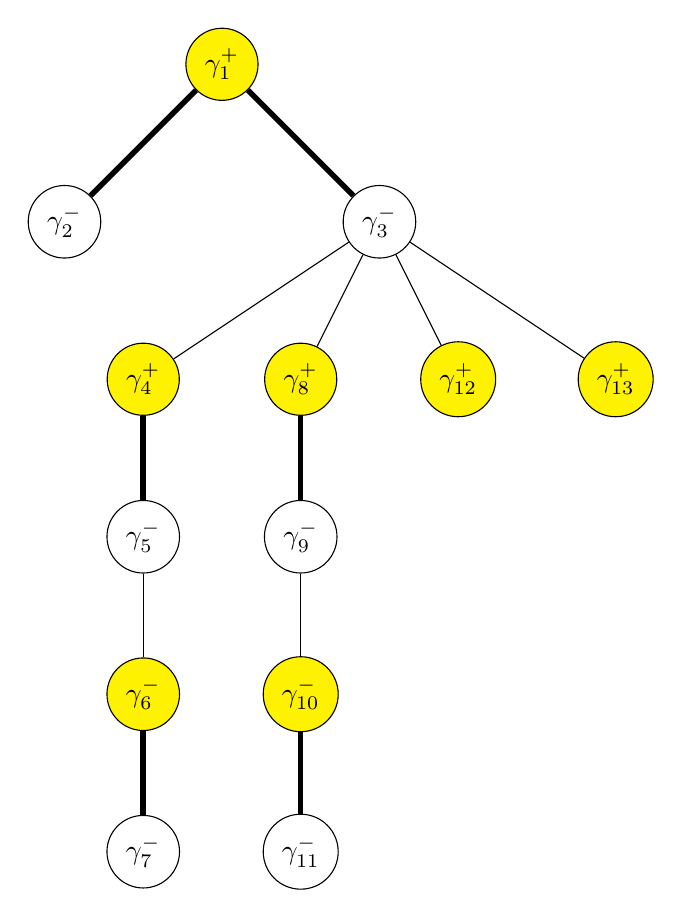
\begin{tikzpicture}
			\node[circle,draw,fill=yellow](n1) at (0,0){$\gamma_1^+$};
			\node[circle,draw](n2) at (-2,-2) {$\gamma_2^-$};
			\node[circle,draw](n3) at (2,-2) {$\gamma_3^-$};
			\node[circle,draw,fill=yellow](n4) at (-1,-4) {$\gamma_{4}^+$};
			\node[circle,draw,fill=yellow](n8) at (+1,-4) {$\gamma_8^+$};
			\node[circle,draw,fill=yellow](n12) at (+3,-4) {$\gamma_{12}^+$};
			\node[circle,draw,fill=yellow](n13) at (+5,-4) {$\gamma_{13}^+$};
			\node[circle,draw](n5) at (-1,-6) {$\gamma_5^-$};
			\node[circle,draw,fill=yellow](n6) at (-1,-8) {$\gamma_6^-$};
			\node[circle,draw](n7) at (-1,-10) {$\gamma_7^-$};
			\node[circle,draw](n9) at (1,-6) {$\gamma_9^-$};
			\node[circle,draw,fill=yellow](n10) at (1,-8) {$\gamma_{10}^-$};
			\node[circle,draw](n11) at (1,-10) {$\gamma_{11}^-$};
			\draw[line width=2] (n1)--(n2);
			\draw[line width=2] (n1)--(n3);
			\draw[line width=2] (n4)--(n5);
			\draw[line width=2] (n6)--(n7);
			\draw[line width=2] (n8)--(n9);
			\draw[line width=2] (n10)--(n11);
			\draw (n3)--(n4);
			\draw (n3)--(n8);
			\draw (n3)--(n12);
			\draw (n3)--(n13);
			\draw (n5)--(n6);
			\draw (n9)--(n10);	
		\end{tikzpicture}
		\caption{Hasse diagram}
	\end{figure}

	\subsection{Spadjor表示}
	根据论文中的思路,我们给出本文中卡通图案对应的Spadjor表示法。
	
		$\mathcal{J}=\{\gamma_{1}^{+},\gamma_{2}^{-},\gamma_{3}^{-},\gamma_{4}^{+},\gamma_{8}^{+},\gamma_{12}^{+},\gamma_{13}^{+},\gamma_{5}^{-},\gamma_{6}^{+},\gamma_{7}^{-},\gamma_{9}^{-},\gamma_{10}^{+},\gamma_{11}^{-}\}$
		
		$\mathcal{J}=\cup_{k=1}^{7}\mathcal{J}_k$
		
		$\mathcal{J}_1=\{\gamma_{1},\gamma_{2},\gamma_{3}\}$,$\mathcal{J}_2=\{\gamma_{4},\gamma_{5}\}$,$\mathcal{J}_3=\{\gamma_{6},\gamma_{7}\}$,$\mathcal{J}_4=\{\gamma_{8},\gamma_{9}\}$,$\mathcal{J}_5=\{\gamma_{10},\gamma_{11}\}$,$\mathcal{J}_6=\{\gamma_{12}\}$,$\mathcal{J}_7=\{\gamma_{13}\}$.
		
		$\mathcal{Y}=\cup_{k=1}^{7}\mathcal{Y}_k=\rho(\mathcal{J})$,$\mathcal{Y}_k=\rho(\mathcal{J}_k)$
		
		$\mathcal{Y}=\cup_{k=1}^7\mathcal{Y}_k=[\cap_{i=1}^{3}int(\gamma_{i})]\cup[\cap_{i=4}^{5}int(\gamma_{i})]\cup[\cap_{i=6}^{7}int(\gamma_{i})]\cup[\cap_{i=8}^{9}int(\gamma_{i})]\cup[\cap_{i=10}^{11}int(\gamma_{i})]\cup int(\gamma_{12}) \cup int(\gamma_{13})$
	
		
	\newpage
	\section{Yin集合上的布尔代数}
	\subsection{一种朴素的实现方法}
	\subsubsection{多边形填充——扫描线算法}
	此部分基于\verb|Visual Studio 2019|平台,使用的图形库是\verb|EasyX|,主要用到的算法是扫描线算法,用于多边形填充。一般来讲,本算法实现过程中会用到两个数据结构:边表、活动边表。给定一扫描线,其对应的$ET$表,即边表,主要由四部分构成:某边的纵坐标最大值、最小值,最小值对应的横坐标、某边的斜率。
	
	
	在建立$ET$表后,开始扫描转换。不同的扫描线与之相交的边线也不同,当扫描线进行转换时,我们需要考虑其对应的相交的边线,由此我们需要建立一个活动边表$AET$。
	
	在对图案进行遍历扫描时,我们对每个$y$值都设置了一个数组,用以存放该扫描线与边线相交的横坐标值,并在得到所有横坐标值后对其进行排列。
	
	进行上述操作后我们对每一个$y$都得到了存放交点坐标值的数组$x[stack]$,此时只需要设置步长为2进行遍历,将坐标点用特定颜色两两连线,全部操作结束即完成对多边形区域染色。需要说明的是,一般来讲交点数均为偶数,即使有一些特殊情况,例如与极值点相交、扫描线经过某边等情况,也都已经在算法具体代码实现过程中给出了相应的解决方案。
	
	以上便是程序中函数\verb|draw_Polygons1|和\verb|draw_Polygons3|的主要思路,而对于其余几个函数,也只是在染色这一步骤中的具体实现方法有细微差别,具体的思路为:在$x[stack]$两两配对后的序列中对$x$进行逐点遍历,利用\verb|getpixel|函数获取该点颜色信息,然后根据不同情况进行区域填充(不再对线条染色而直接对区域染色),遇到边界即停止染色。需要说明的一点是,图案的边界曲线已提前绘制,只需利用传入各函数的坐标参数连线绘制即可。
	
		
	\subsubsection{程序及结果}
	在本题中,我们首先将两幅图用$\mathcal{J}$的形式表示。对于熊猫,可表示为$\mathcal{J}=\cup_{k=1}^{6}\mathcal{J}_k$,其中$\mathcal{J}_1=\{\gamma_{1}^+,\gamma_{2}^-,\gamma_{3}^-\}$,$\mathcal{J}_2=\{\gamma_4^+,\gamma_5^-\}$,$\mathcal{J}_3=\{\gamma_6^+,\gamma_6^-\}$,$\mathcal{J}_4=\{\gamma_8^+\}$,$\mathcal{J}_5=\{\gamma_9^+\}$,$\mathcal{J}_6=\{\gamma_{10}^+\}$.对于米老鼠,可表示为$\mathcal{J}=\cup_{k=1}^{2}\mathcal{J}_k$,其中$\mathcal{J}_1=\{\gamma_{1}^+,\gamma_{2}^-,\gamma_{3}^-,\gamma_{4}^-\}$,$\mathcal{J}_2=\{\gamma_5^+,\gamma_6^-\}$.
	
	若要得到某单个图案,我们只需要重复利用定义的函数\verb|draw_Polygons1|
	和\verb|draw_Polygons3|反复对正向曲线和反向曲线围成的区域染色即可。
	
	\begin{figure}[!h]
		\centering 
		\subfigure[Panda]{
			\label{Fig.sub.1}
			\includegraphics[width=0.35\textwidth]{P.jpg}}
		\subfigure[Mouse]{
			\label{Fig.sub.2}
			\includegraphics[width=0.35\textwidth]{M.jpg}}
		\caption{原图案}
	\end{figure}

	若要得到单个图案进行补运算后的图,只需对调两函数即可。
	\begin{figure}[!h]
		\centering 
		\subfigure[Panda的补]{
			\label{Fig.sub.1}
			\includegraphics[width=0.35\textwidth]{P补.jpg}}
		\subfigure[Mouse的补]{
			\label{Fig.sub.2}
			\includegraphics[width=0.35\textwidth]{M补.jpg}}
		\caption{原图的补运算}
	\end{figure}
	
	若要得到两图的交或并,我们首先确定一块主区域。假定我们选定熊猫作为主区域,先重复上述操作,此时我们在过程上得到了熊猫的图案。此时,我们只需要对构成米老鼠的每一个$\mathcal{J}_k$调用相应的函数,函数原理与此前提到的两个函数相似,不过输入参数增加至多条曲线的特征点,$x[stack]$的计算过程更为复杂。

	在此部分的函数中,我们加入了检测该区域颜色的操作,便于交并运算的实现。若某区域属于熊猫图而不属于米老鼠图,则保持原色不变;若不属于熊猫图而属于米老鼠图,则染为其他一种颜色;若某块区域既属于熊猫图又属于米老鼠图,则染为另一种颜色。
	
	\begin{figure}[!h]
		\centering
		\includegraphics[width=0.5\textwidth]{P和M.jpg}
		\caption{交并运算的中间过程图}
	\end{figure}

	\newpage
	在进行上述操作后,我们得到了四个不同颜色的区域:$(P\cup^{\bot\bot} M)^{\bot}$、$P\cap M$、$P\cap M^{\bot}$、$M\cap P^{\bot}$。若要得到两图交运算后的图,我们只需要保留两图共有的区域,即$P\cap M$;若要得到两图并运算后的图,我们只需要将$P\cap M$、$P\cap M^{\bot}$、$M\cap P^{\bot}$三部分染为一种颜色。
	
	\begin{figure}[!h]
		\centering 
		\subfigure[Panda与Mouse的交]{
			\label{Fig.sub.5}
			\includegraphics[width=0.4\textwidth]{P交M.jpg}}
		\subfigure[Panda与Mouse的并]{
			\label{Fig.sub.6}
			\includegraphics[width=0.4\textwidth]{P并M.jpg}}
		\caption{P和M的交与并}
	\end{figure}

	需要说明的一点是,在本部分的程序中浮点数坐标读入后全部转换为整型参与运算,这是因为我们坐标系取得足够大,浮点数带来的误差几乎可以忽略。

	\subsection{论文的实现思路}
	上述的算法是一种比较朴素的图在进行交并补运算后呈现结果的实现方法。严格来讲,上述算法并没有实现对Yin集合的布尔代数运算。在询问邱助教后,我明白题目所希望的布尔代数是利用算法对Yin集合实现各种运算,其输入和输出的形式应该是近乎相同的,这种运算的封闭性是论文的价值所在,也是大作业的难点所在。
	
	虽然没有完整地实现这种想法,但也有了一定的解决思路。首先是语言方面,我在本次大作业的编程语言上选择了C语言,但我认为采用C++对于本部分会更方便便捷。要实现Yin集合的封闭运算,自然而然地想到定义封装一些类,然后对类进行相应操作。
	
	我认为本文中上述提到的多边形扫描线算法,在此种方法的实现里也是能利用的,并且也是一个非常关键的部分,利用这种方法在两个多边形运算操作后得到新的多边形,这里多边形均通过边或者点的信息来记录和表示。不过很遗憾,我意识到这一点比较晚,且在思考后认为这种方法超出了目前我的能力范围,因此最终没有完成这种算法。

	\section{结语}
	本次大作业很好地锻炼了我的编程能力,也在一定程度上提升了我面对某个陌生问题时举一反三、自主设计算法进行解决的能力。在完成本次作业后,对暑期课程中提到的一些重难点有了切身的认识和体会,也更明白了论文的价值所在。总体而言,虽然尚有缺憾之处,但仍十分有成就感,且收获颇丰。
	
\end{document}
